%!TEX encoding = UTF-8 Unicode
%!TEX root = ../main.tex

\chapter{Software Requirements in Context}
There is a theory which states that if ever anyone discovers exactly what the Universe is for and why it is here, it will instantly disappear and be replaced by something even more bizarre and inexplicable.
There is another theory which states that this has already happened. \cite{lauesen2001software}

\begin{figure}[h!]
\centering
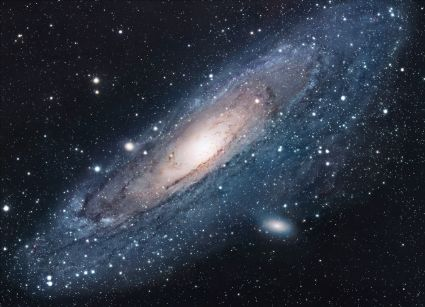
\includegraphics[scale=1.7]{./img/universe.jpg}
\caption{The Universe}
\label{fig:universe}
\end{figure}


\section{What is a Requirement?}

\begin{itemize}
  \item Different kinds of requirements
  \item Requriements at different levels
  \item Goal-design-scale
  \item The Feature as a decision unit
  \item Requirements as ideas, decisions, system properties, ...
  \item Quality vs function
\end{itemize}

\section{What is Requirement Engineering?}


\subsection{Sub-processes of Requirements Engineering}

\begin{itemize}
  \item Invent: Elicitation
  \item Persist: Specification
  \item Check: Validation
  \item Decide: Prioritize
  \item Plan: Management
\end{itemize}

\subsection{Requirements Engineering in different project types}

\begin{itemize}
  \item Procurement, private versus public procurement, tender processes
  \item Product development for a market
  \item Bespoke development for a single customer
  \item In-house development for our own use
  \item Community development and open source
\end{itemize}

\subsection{Requirements in the Software Development Process}

\begin{itemize}
  \item Evolution: from inception to migration in the software development lifecycle
  \item Decision-making and change control
  \item Configuration management, git
  \item Increments, commits and releases
  \item Software hosting and issues as requriements
  \item RE and Testing
  \item RE and System Architecture
  \item RE and SW Design, UX, HCI, Usability...
  \item RE and Project Management
  \begin{itemize}
    \item states of requriements (-> Release Planning)
    \item funnel from ideas to implementation
  \end{itemize}
   \item RE and System Operation (Devops, feedback loops, continuous deployment etc)
   \item RE as a communication process, Communication distances
\end{itemize}

\subsection{Requirements in Systems Engineering}

\begin{itemize}
  \item Human-centric systems: Desktop apps, Webb apps
  \item Embedded systems
  \begin{itemize}
    \item Hardware and Software Co-design
    \item Internet of things
  \end{itemize}
  \item Safety-critical systems
\end{itemize}

\section{Ethics in Requirements Engineering}

\begin{itemize}
  \item Systems that are friendly to users and their planet
  \item Systems that spy on humans
  \item Systems that may kill humans
  \item Engineering ethics frameworks
\end{itemize}
